% !Mode:: "TeX:UTF-8"

\chapter{ss方程守恒律程序包开发}
本论文中的第二章主要介绍了研究过程中所使用的基础的数学方法,第三章和第四章介绍了论文研究中的主要内容。在研究过中因为涉及到了大量的数学计算、公式推导和方程求解,纯人工操作会因计算量过大以及各种可能的错误而不太可靠,因此我们不得不借助符号计算工具 Mathematica,编写基于 Wolfram 的语言的程序来去辅助计算和研究。然而由于本论文数学研究的特点以及 Mathematica 软件本身功能的局限性,并不能完全的依靠 Mathematica 软件就能得到研究的结果,往往还需要个人的思考以及人工的操作。在研究本论文内容所编写的 Wolfram 程序一般只能用于该类型的方程的研究,虽然研究方法和思想同样对其它类型的方程研究很有帮助和参考意义,但是程序本身不具有很广的泛化能力。尽管方程研究过程中的计算十分的繁琐并且过程对方程本身的特性和研究方法有很大的依赖性,但仍然有一部分的计算过程是很有规律性或者通用性较好。在这一章中我们试图将这一部分找出来,并将其过程重构为 Mathematica 中 Package 包形式,使得其能够在更多类型的方程研究中发挥更好的作用。

在本文中的第二章第三节中介绍了偏微分方程的守恒律的基础数学知识,守恒律作为非线性偏微分方程中一个很重要的性质,对于研究非线性偏微分来说具有很重要的作用。然而,求解偏微分方程守恒律的过程并不是一成不变的,一般来说不同类型方程的求解方式会具有很大的差异,在求解的过程中,往往只能凭借研究人员的个人的思考和过往研究经验对中间过程进行人工处理,才能得到最终的结果。幸运的是,在求解方程守恒律的过程中并不是所有的步骤都需要人工式的处理,仍然有一些步骤是机械式的流程,对于不同类型的方程,只要给出足够必要的条件,就能不断的迭代产生出从第一项到任意一项的守恒律。以 Sasa-Satsuma 方程为例,首先得到目标方程分别关于时间和空间多项式 $D_n$ 和 $F_n$ 的表达式,然后再得到表达式中依赖项的形式和起始项,就很容易的可以推导出任意一项的守恒律,最后进行验证是否正确。 因此可以将这一部分流程抽象出来,编写出用于求解守恒律的程序包。本章将主要介绍使用 Mathematica 内置的编程语言 Wolfram 来封装求解守恒律过程的程序包。

\section{Wolfram Mathematica 基本介绍}
Mathematica 是一款用于符号计算的软件,也被称为计算机代数系统,广泛用于科学研究、工程、数学计算等领域, 同时也是目前使用最为广泛的数学软件之一。而 Wolfram 语言是用于 Mathematica 的编程语言,它的用法和其它的高级编程语言有着很大的不同。Wolfram 集合了大量的编程模式,并使用独特的符号编程理念,是一种基于知识的语言,在编程上具有很大的灵活度。它使用各种语法规则去解释输入,使用标准输入框将字符串或框符转化为表达式。Wolfram 是一种交互式的编程语言,使用时只需敲入输入,然后按 SHIFT+ENTER 便可进行计算得到结果\upcite{syc-5}。下面将简要的介绍 Wolfram 语言中最基础的语法和概念。
\begin{itemize}
    \item 表达式
\end{itemize}

在 Wolfram 语言中,一切都是符号表达式。尽管 Wolfram 语言可以处理多种不同形式的对象,例如数学公式、列表、图形等,它们在形式上看起来有所不同,但是 Wolfram 语言以统一的方式来表达它们。符号表达式可以进一步的划分为两种类型:原子表达式和普通表达式。原子表达式是组成表达式中最小单元,主要包括数字、分数、实数、复数、符号、字符串等。普通表达式由原子表达式组成,所有的普通符号表达式都具有相同的基本结构:$head[arguments]$

${a, b, c} \cdots List[a, b, c]$

$2 + 2 \cdots Plus[2, 2]$

其中 $head$ 是表达式的头部, $arguments$ 表示表达式的参数,参数也可以是任何符号表达式,例如

$x^2 + 3y^3 \cdots Plus[Power[x, 2], Times[3, Power[y, 3]]]$

\begin{itemize}
   \item 列表
\end{itemize}

列表是 Wolfram 语言的一种重要的数据结构,可以用来表示各种类型的集合、数组以及序列。在 Wolfram 语言中,列表可以是任意的结构和大小,甚至能够包含数百万个元素。 Wolfram 语言中可以直接在列表上进行操作的函数超过 1000 个,这使得列表成为 Mathematica 中一个协同工作的强大工具。在 Wolfram 语言中列表用 $\{\cdots\}$ 表示,其中的元素可以是任何类型的表达式。列表部分的索引从 1 开始,可以使用 $[[\cdots]]$ 进行提取,而负索引从列表的结尾向前开始计数,例如

$\{a, b, c\}[[3]]$ 的结果是 $c$,

$\{a, b, c, d, e, f\}[[-3]]$ 的结果是 $d$。

\begin{itemize}
    \item 函数
\end{itemize}

Wolfram 系统的符号语言模式,将变量和函数的定义提高到了一个新的层次。 在 Wolfram 系统中,变量不仅可以代表一个数值,而且可以作为一个纯粹的符号来使用。基于 Wolfram 系统强大的模式语言, “函数” 定义不仅仅是变量,而且可以转换为任意结构的模式。在 Wolfram 语言中,函数定义只是给出模式变换规则的复制,例如定义一个带有命名为 $x$ 和 $y$ 两个参数的函数

$f[x\_ , y\_ ]:= x + y$

使用上述定义

$f[4, a]$ 输出结果是 $4 + a$.

通常情况下,Wolfram 语言一般假设变量是全局变量. 即每次使用  $x$ 等名字时,Wolfram 语言总认为在调用同一对象。然而在编程时,不需要将所有变量都作为全局变量。例如,在两个不同的程序中,$x$ 可用来指代两个不同的变量. 此时,每个程序中的 $x$ 都必须作为局部变量。为了解决这个问题,在 Wolfram 语言中可以使用  Modules 定义局部变量,

$f[x\_ , y\_ ]:= (Module[\{x, y, \cdots\}, body])$

其中 $x, y$ 是局部变量,$body$ 处为具体的函数体

除了可以自定义函数外,Wolfram 语言还提供近 5000 个内置函数共用户使用,一般每个内置函数名称的首字母均为大写。这些内置函数会大大的简化程序编写的工作量,下面给出一些常用到的内置函数

$\mathrm{Simplify[expr]}$  \quad   化简表达式 $expr$

$\mathrm{Expand[expr]}$ \quad    展开表达式 $expr$ 的每一项

$\mathrm{Solve[expr, vars]}$  \quad 求解以 $vars$ 为变量的方程组或不等式组 $expr$

$\mathrm{DSolve[eqn, u, x]}$ \quad  为函数 $u$ 求解微分方程,$x$ 为独立变量

$\mathrm{DSolve[\{eqn_1, eqn_2, \cdots \}, \{u_1, u_2, \cdots \}, \cdots ]}$ \quad  用来求解一系列微分方程

$\mathrm{D[f,x]}$     \quad  关于函数 $f$ 对 $x$ 求微分

$\mathrm{D[f,{x,n}]}$     \quad     关于函数 $f$ 求 $x$ 的 $n$ 阶微分

$\mathrm{Coefficient[expr, form]}$   \quad  给出了多项式 $expr$ 中 $form$ 的系数

$\mathrm{CoefficientList[poly, var]}$   \quad  给出在 $poly$ 中 $var$ 的幂系数的列表,从 0 次幂开始

\section{守恒律的求解实现}
根据本论文的第三章和第四章的研究内容发现,求解守恒律的过程有相当一部分步骤的形式是一样的,尽管这两个方程之间还存在着微小的差距,但是这些差距仅仅是最基本函数形式不同,不会影响到守恒律的求解过程,因此这一小节我们将其中的公共部分抽取出来来编写适用性更广的程序。
\subsection{依赖项系数的实现}
如果知道一个微分方程的守恒律的表达式以及表达式依赖项的形式和起始项,那么我们就可以求出该方程任意一组的守恒律。当然首先是需要得到守恒律通项公式的依赖项系数的形式和起始项。从论文中的第三章和第四章内容我们发现依赖项系数很多但大部分的形式相似度很高,最主要是先获得依赖项 $c_n$ 和 $d_n$ 的形式。为了能够同时应用于两个方程中,我们将依赖项系数以列表的形式传入,而不是以表达式的形式。

附录 A 是代码的简单实现,代码中 $getGeneralTerm$ 函数接收五个参数,$c1$ 是守恒律表达式所依赖项系数 $c_n$ 的第一项, $d1$ 是守恒律表达式所依赖项系数 $d_n$ 的第一项,$coe1$ 表示对应系数的函数列表,$co2$ 对应系数的函数其它形式列表,一般情况下是共轭形式,$n$ 表示想要得到第几组的序号。程序的内部过程是通项公式 $c_n$ 和 $d_n$ 的求解过程,在本论文中形式比较固定,它们的表达式的具体形式如下所示
\begin{align}
  & c_{n+2} = \frac{1}{2a\mathrm{i}} \left[c_{n+1,x} + a\sum_{m=0}^{n+1}(c_{m}c_{n+1-m}ku^{*} + c_{m}d_{n+1-m}k^{*}u)\right] \\
  & d_{n+2} = \frac{1}{2a\mathrm{i}} \left[ d_{n+1,x} + a\sum_{m=0}^{n+1}(d_{m}d_{n+1-m}k^{*}u + d_{m}c_{n+1-m}ku^{*}) \right]
\end{align}
在论文中对于数列 $c_n, d_n$ 只有首项和一些系数函数会因为不同的方程而不同,它作为参数被传入到代码中的函数,因此只要知道首项的形式就很容易推导出任意一项的结果。

\begin{figure}[!htp]
	\centering
	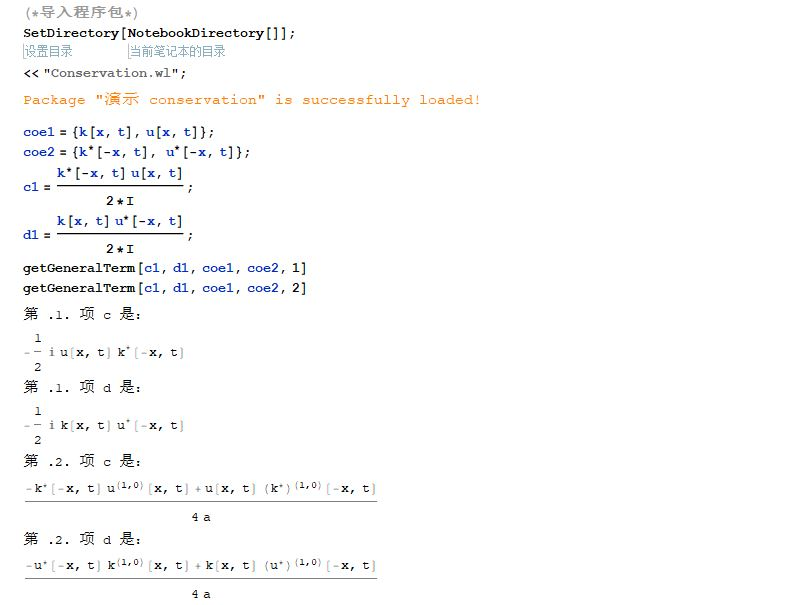
\includegraphics[width=0.97\linewidth]{getGeneralTerm.jpg}
	\caption{求解依赖项的运行结果}
	%with same parameters~$k=1 , \alpha_2(t)=1, \alpha_0(t)=0$.
	\label{picture-5-1}
\end{figure}
下面是对程序的使用过程的介绍:如果想要使用该程序,首先导入封装该函数的程序包 $Conservation.wl$,以 .wl 为后缀的文件是 Mathematica 所提供的自定义程序包的文件格式。如果加载程序包后出现 $Package \ "Conservation" \ is \ successfully \  loaded!$ 的输出语句说明程序包加载成功。然后就可以调用程序包中的函数,运行结果如图 \ref{picture-5-1} 所示。该图只展示了所得到$c_n, d_n$ 前两项的结果。可以看到,图 \ref{picture-5-1} 的运行结果和第四章第三节中得到的结果是一致的。


\subsection{守恒律求解的实现}
在实现依赖项求解之后,接下来的问题就是如何求解方程的守恒律。和上一小节的过程类似,我们在得到方程守恒律的通项公式后,就可以很容易的求得任意项的守恒律,这些通项公式中的一些参数系数部分是上一小节求得的结果,另一部分是固定形式的参数,它们被当作变量传入到代码的函数中。为了能够同时适应两个方程,参数都是以列表的形式传入,而不是单一的表达式。

附录 B 是代码的简单实现,代码中 $Conservation$ 函数接收五个参数,$clist$ 是上一小节得到的 $c_n$ 前 $n$ 项的列表,而$dlist$ 是则是上一小节中的得到的 $d_n$ 的前 $n$ 项列表,$coe1$ 表示对应系数的函数列表,$co2$ 对应系数的函数其它形式列表,一般情况下是共轭形式,$n$ 表示想要得到第几组守恒律。程序的内部过程是关于 Sasa-Satsuma 类型方程的守恒律的求解过程。其中守恒律中的 $D_n$ 和 $F_n$ 项的表达式如下所示,
\begin{align}
  & D_{n} = a(ku^{*}c_{n} + k^{*}ud_{n}) \\
  & F_{n} = b(t)\left[A_{2}kc_{n+1} + A_{4}kc_{n} + \frac{2}{3}ku^{*}c_{n+2} + \frac{2}{3}uk^{*}d_{n+2} - A_{2}^{*}k^{*}d_{n+1} + A_{4}^{*}k^{*}d_{n}\right]
\end{align}
对于 Sasa-Satsuma 类型的方程守恒律的求解基本上都可以通过上述的方程来求得,因此只要指导表达式中对应元素的形式就能求得其中任意组的守恒律。而表达式中的元素 $A_2, A_4, k$ 等根据方程的不同可能会有不同的形式,$c_n, d_n$ 的形式相对固定,并且求解过程在上一小节中已给出。下面介绍该函数的使用过程和运行结果。

使用上述代码之前需要调用上一小节中的代码。以本论文中的第四章研究的方程 (\ref{nss-1}) 为例,运用上述函数求得方程 (\ref{nss-1}) 的守恒律:首先导入封装该函数的程序包 $Conservation.wl$,加载程序包后出现 $Package \ "Conservation" \ is \ successfully \  loaded!$ 表示加载成功。然后就可以调用程序包中的 $getGeneralTerm$ 函数,并在该函数的内部调用 $Conservation$,并传入相应的参数。运行结果如图 \ref{picture-5-2} 所示。这里我们只运行给出了方程 (\ref{nss-1}) 的第一组守恒律的结果。可以看到守恒律的结果和第四章第三节中的结果是一致的。
\begin{figure}[!htp]
\centering
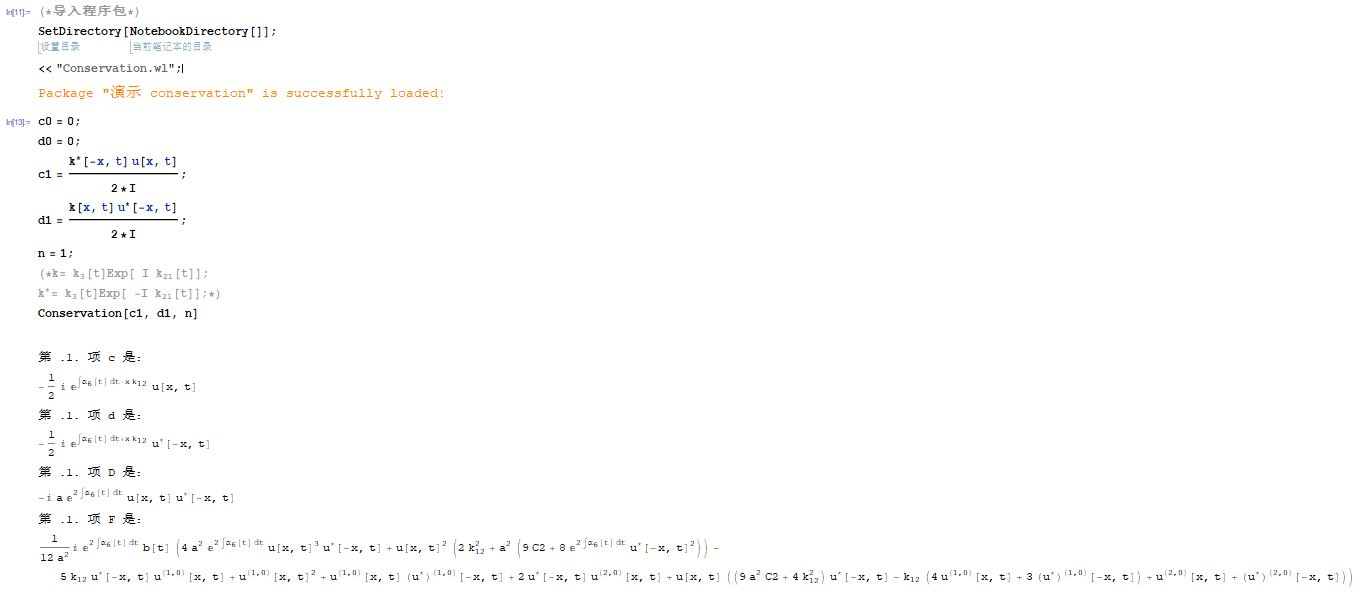
\includegraphics[width=\linewidth]{getConservation.jpg}
\caption{求解方程的守恒律}
%with same parameters~$k=1 , \alpha_2(t)=1, \alpha_0(t)=0$.
\label{picture-5-2}
\end{figure}

\section{验证守恒律}
上一节实现了用于求解方程守恒律的程序,接下来这一节对得到的守恒律进行验证,然而不像求解守恒律那么般有规律,不同组的守恒律验证往往又不一样,因此目前程序只对前两组守恒律进行验证。

附录 C 中的 $validateConservation$ 函数接收 8 个参数, $equ1, equ2$ 分别表示所研究的目标方程和目标方程的共轭形式,$u, v$ 分别是方程中的原子函数及其的共轭函数,即 $equ1, equ2$ 都是关于函数 $u, v$ 的非线性偏微分方程。$d, f$ 是前一步中求得的一组守恒律。$n$ 表示传入进来的守恒律是第几组,$c$ 表示一个不含函数 $u[x,t]$ 和其共轭函数的常数项。验证的思路如下:将守恒律中 $d$ 项函数对 $t$ 进行求导,对守恒律中 $f$ 项函数对 $x$ 求导,两者的结果相减,如果结果等于 0,那么守恒律就成立。但是一般相减后结果仍然是一个关于函数 $u$ 的多项式,如果它能与研究的目标方程等价,那么结果也就自然等于 0 了。这时,往往对原方程和其共轭方程进行各种形式的变形,使其能够与之前相减的结果等价。对于不同组的守恒律找到的变形往往是不同的,越是往后的守恒律往往形式越是复杂,因此该程序目前是能验证守恒律中前两组相对简单的形式。验证的结果如图  \ref{picture-5-3} 所示,从图中的运行结果我们可以看到方程的前两组的守恒律都成立。

\begin{figure}[!htp]
	\centering
	\subfigure[验证第一组守恒律成立]{
		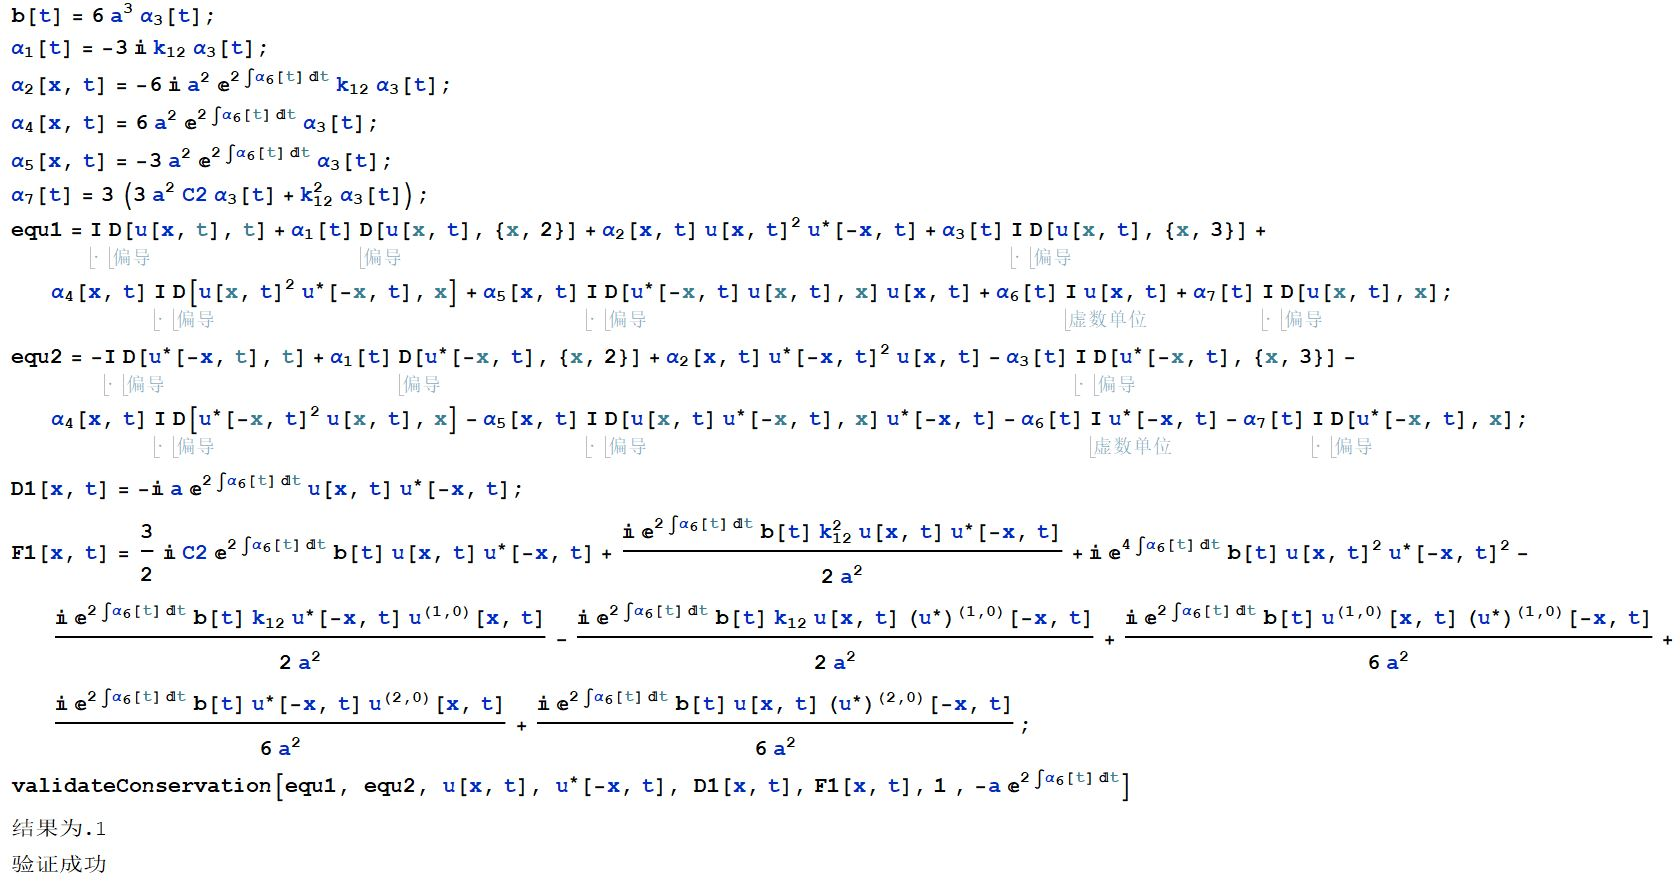
\includegraphics[width=\linewidth]{validateConservation1.jpg}
		\label{picture-5-31}
	}
	\ \
	\subfigure[验证第二组守恒律成立]{
		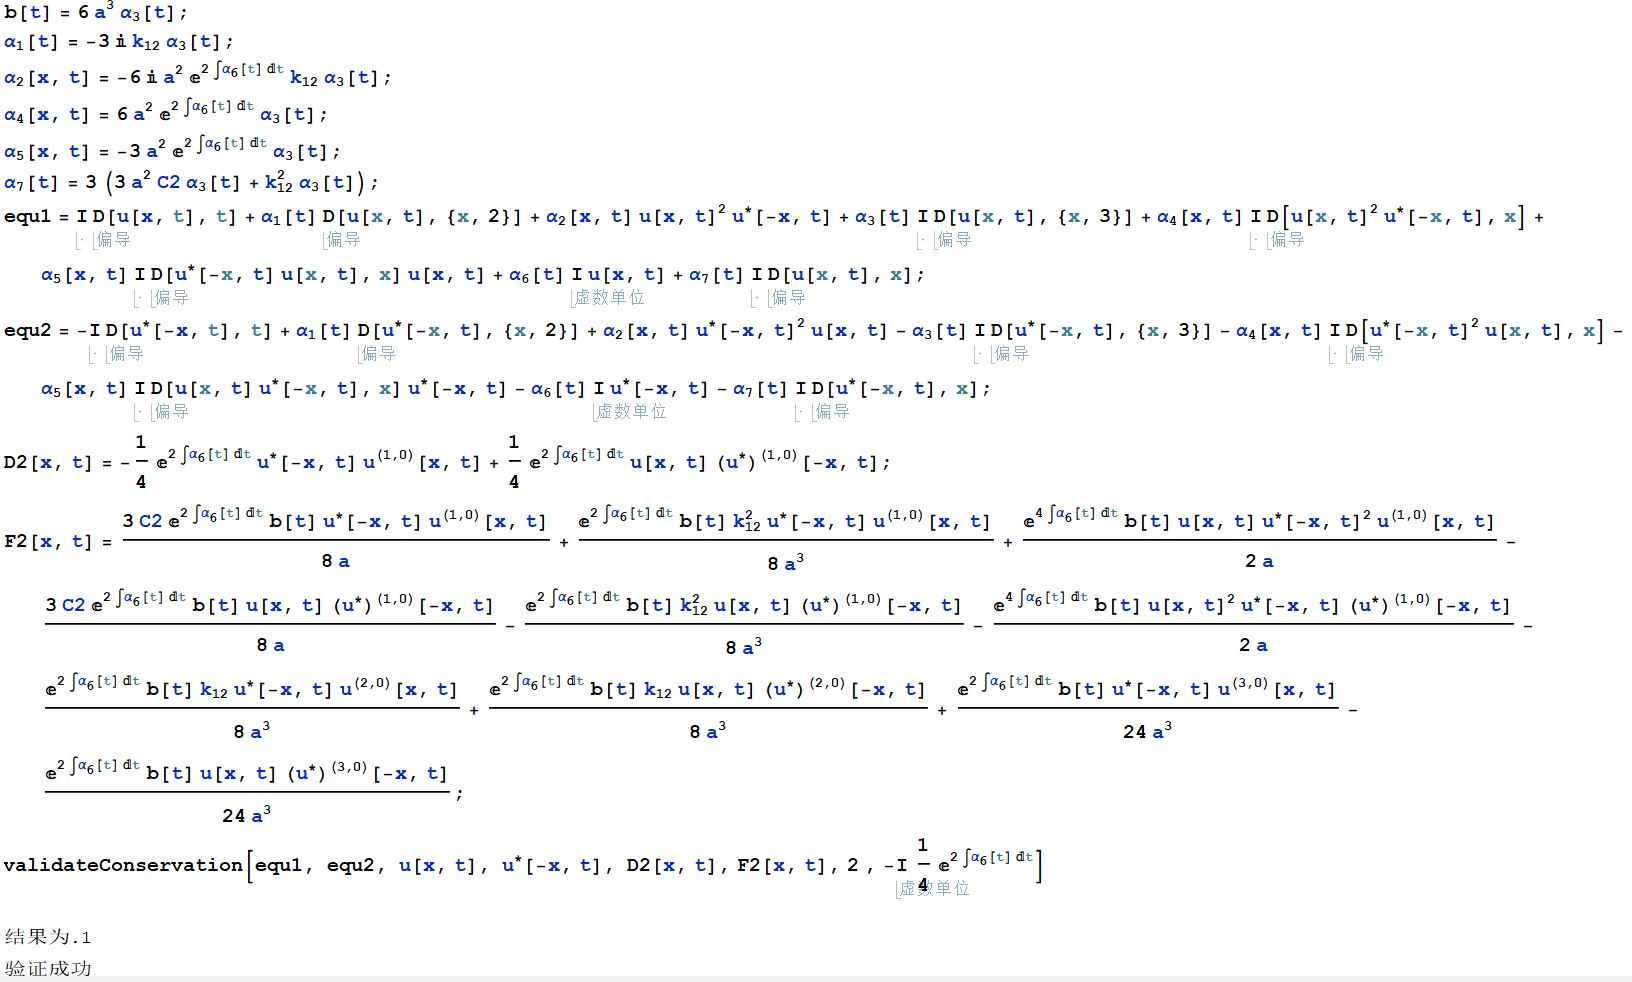
\includegraphics[width=\linewidth]{validateConservation2.jpg}
		\label{picture-5-32}
	}
    \caption{验证守恒律成立}
	\label{picture-5-3}
\end{figure}



\section{本章小结}
本章首先介绍了符号计算软件 Mathematica 的程序编程语言 Wolfram 的基本语法和常用的函数,然后基于 Mathematica 开发了用于得到 ss 方程的守恒律的程序包。这个程序包主要包含两部分的内容,首先是根据方程无穷守恒律的关系表达式迭代推导出前几组的守恒律具体的形式,即 $Conservation$ 函数的实现内容;然后,根据之前得到的守恒律进行验证,验证的方法就是通过寻找方程的各种变形使守恒律达到平衡,即 $validateConservation$ 函数的具体实现内容。最后可以看到本章通过程序包求得的守恒律与第四章求得的守恒律完全一致,并最终通过了验证,这也说明程序包运行的具有较好的正确性和可靠性。


